\section{Feature Selection Experiments}
\label{sec:pmc-results-feature-selection-experiments}

This section investigates the impact of eliminating various shape-derived features on model accuracy, with a particular focus on verifying whether \emph{volume} alone is sufficient to predict peak memory usage.
Section~\ref{sec:pmc-results-model-performance-overview} identified Gradient Boosting, Linear Regression, and Decision Tree as the best performers for Envelope, Gaussian Filter, and \ac{GST3D}, respectively.
Consequently, the experiments below use these three models when removing features.

\subsection{Volume-Centric Hypothesis}
\label{subsec:feature-selection-volume-centric-hypothesis}

Figure~\ref{fig:memory_vs_volume_regression_subplots} shows how tightly memory usage correlates with volume for Envelope, Gaussian Filter, and \ac{GST3D}.
Each subplot includes a regression fit, highlighting that volume on its own explains most of the variance.
This observation motivates a systematic “feature pruning” study to confirm whether additional descriptors (e.g., diagonal length, surface area, ratio features) offer meaningful improvements.

\begin{figure*}[htbp]
    \centering
    \begin{subfigure}[t]{0.32\textwidth}
        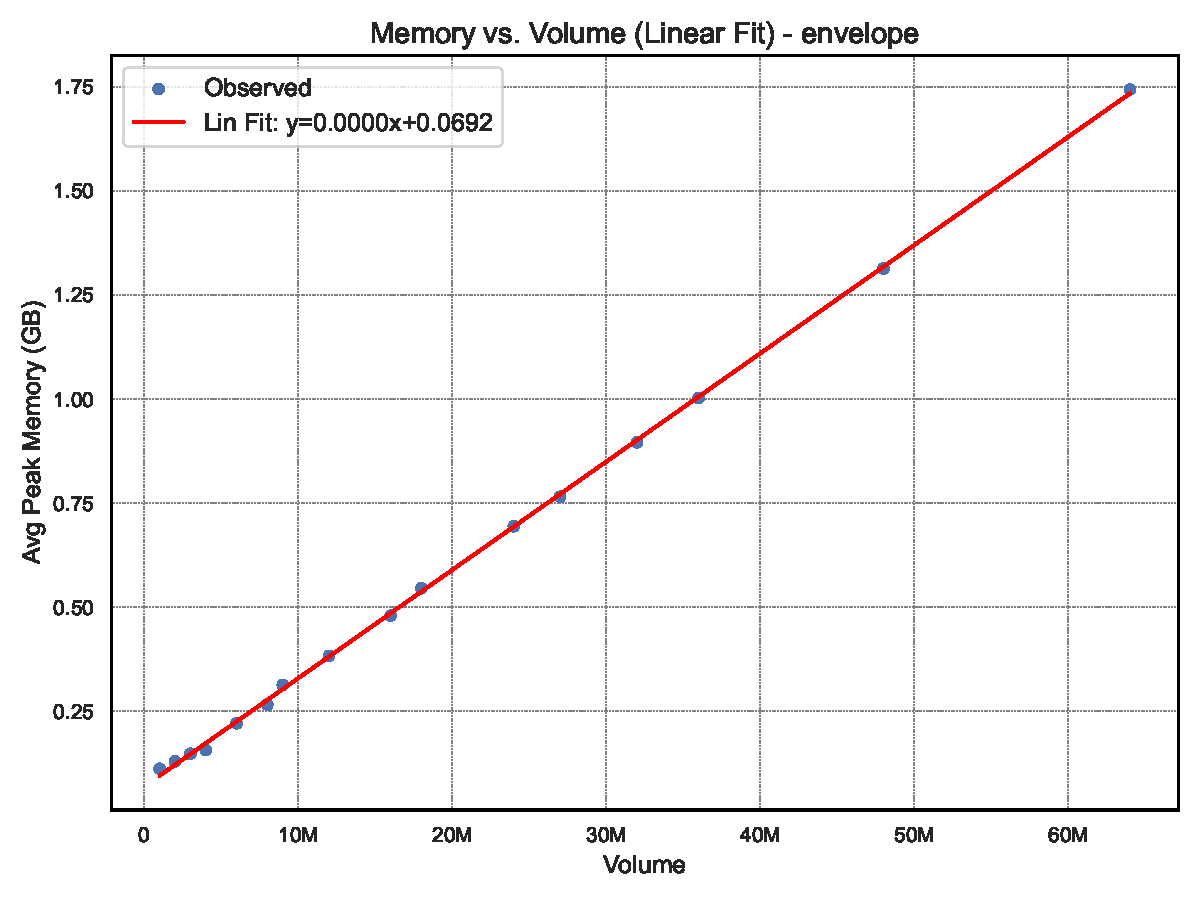
\includegraphics[width=\textwidth]{assets/images/05/memory_vs_volume_regression_envelope}
        \caption{Envelope}
    \end{subfigure}
    \hfill
    \begin{subfigure}[t]{0.32\textwidth}
        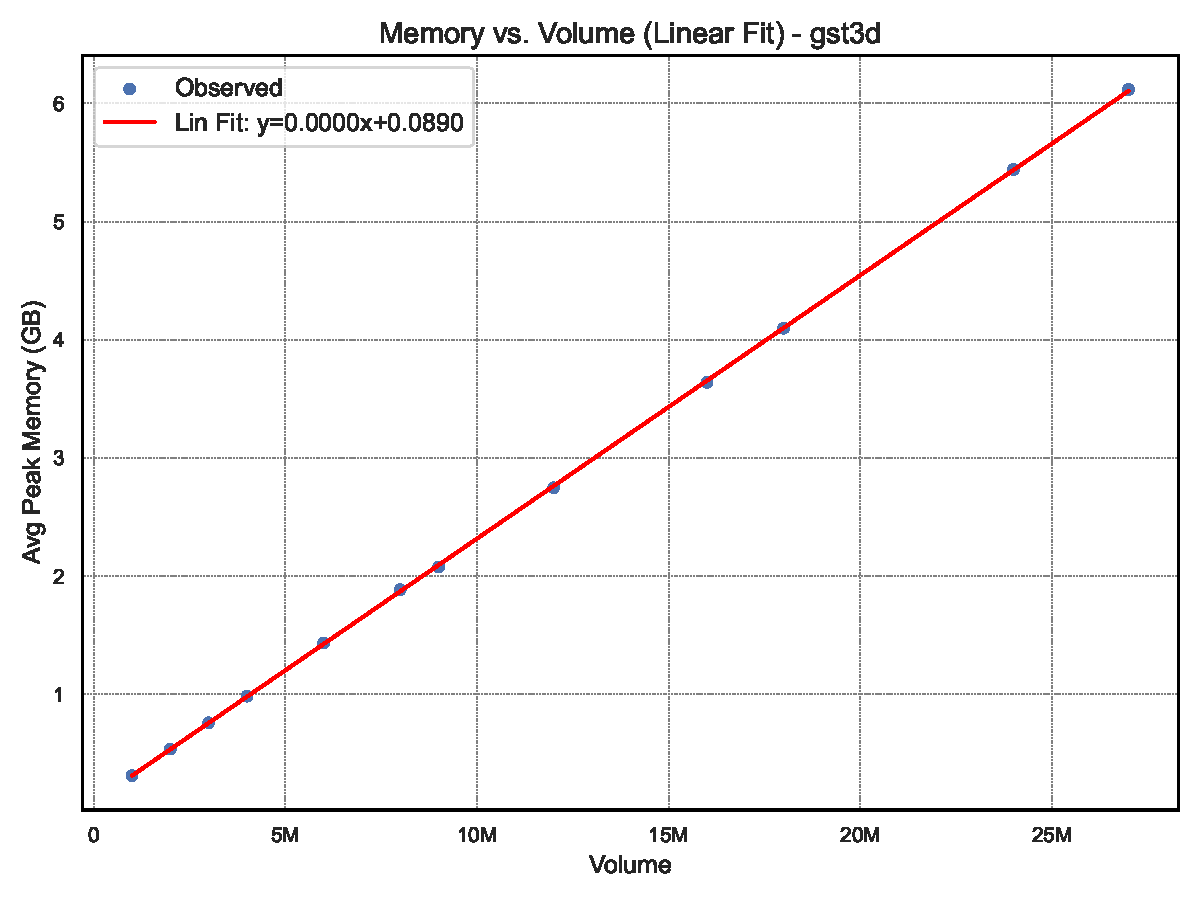
\includegraphics[width=\textwidth]{assets/images/05/memory_vs_volume_regression_gst3d}
        \caption{\ac{GST3D}}
    \end{subfigure}
    \hfill
    \begin{subfigure}[t]{0.32\textwidth}
        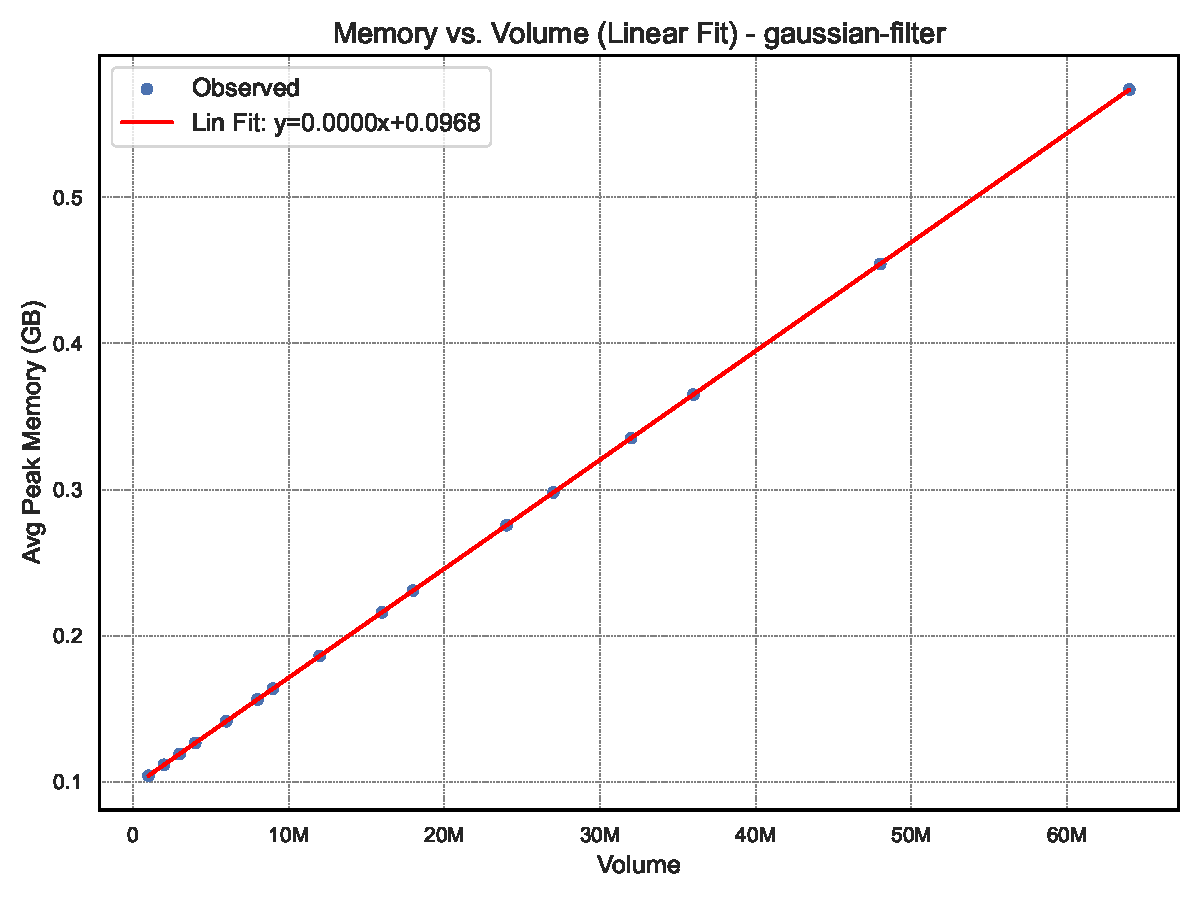
\includegraphics[width=\textwidth]{assets/images/05/memory_vs_volume_regression_gaussian-filter}
        \caption{Gaussian Filter}
    \end{subfigure}
    \caption{Memory usage vs.\ volume with regression lines for Envelope, \ac{GST3D}, and Gaussian Filter.
    All three curves reinforce that volume alone has substantial explanatory power.}
    \label{fig:memory_vs_volume_regression_subplots}
\end{figure*}

\subsection{Feature Removal Process and Metrics}
\label{subsec:feature-removal-methods-and-metrics}

The experiments adopted a stepwise strategy:
\begin{enumerate}
    \item Collect a ranked list of features using a relevance metric (e.g., \emph{SelectKBest}).
    \item Remove the least-relevant feature and retrain the model.
    \item Document changes in \ac{RMSE}, \ac{MAE}, $R^2$, accuracy, and a combined “score.”
    \item Repeat until only \emph{volume} remains.
\end{enumerate}
Table~\ref{tab:feature_selection_minimal_impact} highlights selected examples of Envelope and Gaussian Filter runs, showing how the \ac{RMSE} and $R^2$ shift little upon discarding most auxiliary features.
In nearly all cases, \emph{volume} was never dropped, confirming its primacy in determining memory usage.

\begin{table}[htbp]
    \centering
    \begin{tabular}{lcccccc}
        \hline
        \textbf{Operator} & \textbf{Num.\ Features} & \textbf{Model}    & \textbf{\ac{RMSE}}       & \textbf{$R^2$} & \textbf{Score} & \textbf{Comment} \\
        \hline
        Envelope          & 25                      & Gradient Boosting & 0.0167                   & 0.9961         & 2.5794         & Full set          \\
        Envelope          & 3                       & Gradient Boosting & 0.0150                   & 0.9969         & 2.5823         & Volume + 2 others \\
        \hline
        \ac{GST3D}        & 25                      & Decision Tree     & 0.0023363                & 0.9999970      & 2.9697         & Full set          \\
        \ac{GST3D}        & 3                       & Decision Tree     & 0.0038614                & 0.9999918      & 2.9673         & Volume + 2 others \\
        \hline
        Gaussian Filter   & 25                      & Linear Regression & \(\,2.4 \times 10^{-5}\) & 0.9999999      & 2.9045         & Full set          \\
        Gaussian Filter   & 3                       & Linear Regression & \(\,2.2 \times 10^{-5}\) & 0.9999999      & 2.9045         & Volume + 2 others \\
        \hline
    \end{tabular}
    \caption{Subset of feature-removal results for Envelope, \ac{GST3D}, and Gaussian Filter.
    \ac{RMSE} and $R^2$ remain largely stable as the number of predictors decreases, implying that volume has the dominant role.}
    \label{tab:feature_selection_minimal_impact}
\end{table}

\subsection{Impact on RMSE, R\texorpdfstring{$^2$}{2}, and Residuals}
\label{subsec:impact-on-rmse-r2-and-residuals}

Figures~\ref{fig:feature_selection_overview_part1}--\ref{fig:feature_selection_overview_part2} illustrate the marginal effect of dropping features across operators.
Panel~(a) in Figure~\ref{fig:feature_selection_overview_part1} shows how the \ac{RMSE} changes slightly or not at all when each feature is removed, averaged over multiple runs.
Panel~(b) displays the same logic for $R^2$ scores.
Both metrics exhibit negligible variations except when volume is excluded, which severely degrades performance.

\begin{figure*}[htbp]
    \centering
    \begin{subfigure}[t]{0.49\textwidth}
        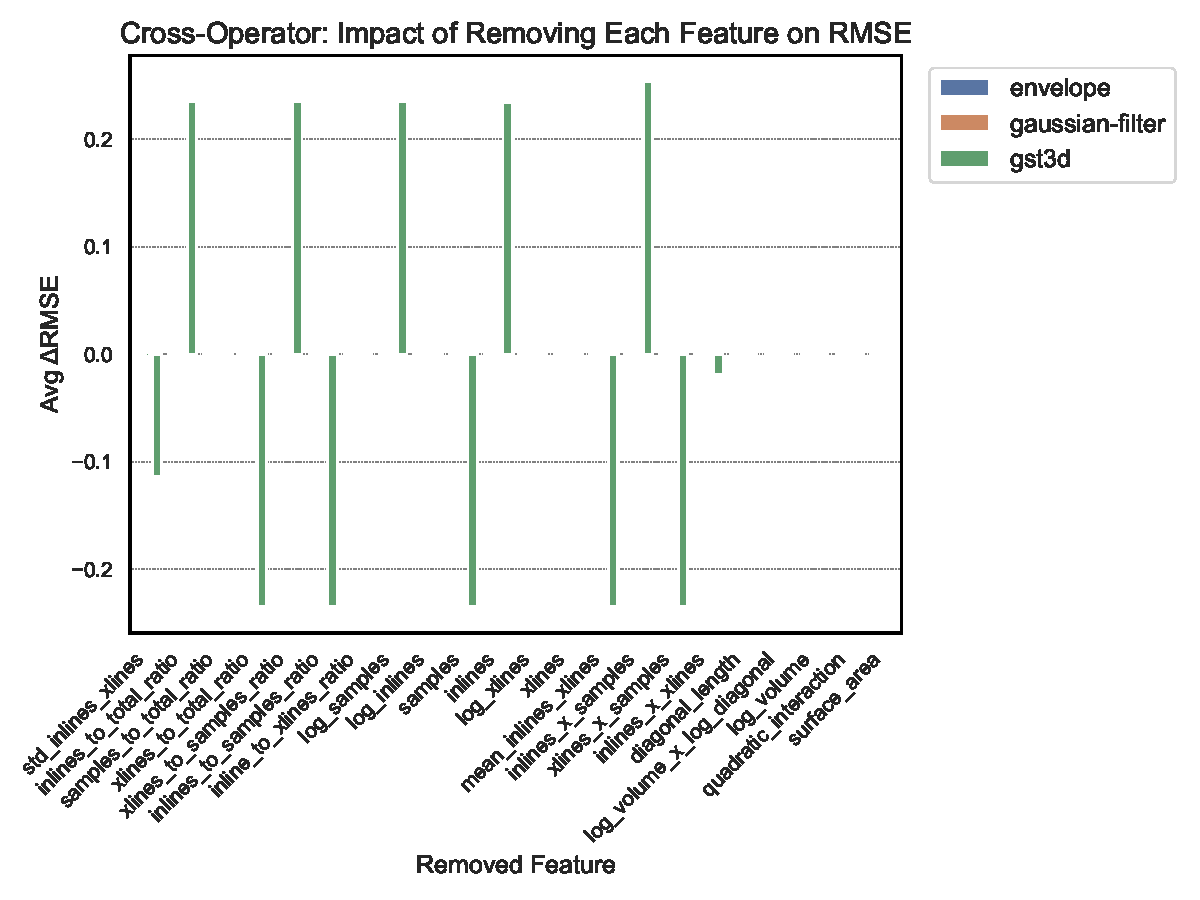
\includegraphics[width=\textwidth]{assets/images/05/feature_impact}
        \caption{Average \ac{RMSE} change per feature removal.
        Smaller bars indicate minimal impact.}
    \end{subfigure}
    \hfill
    \begin{subfigure}[t]{0.49\textwidth}
        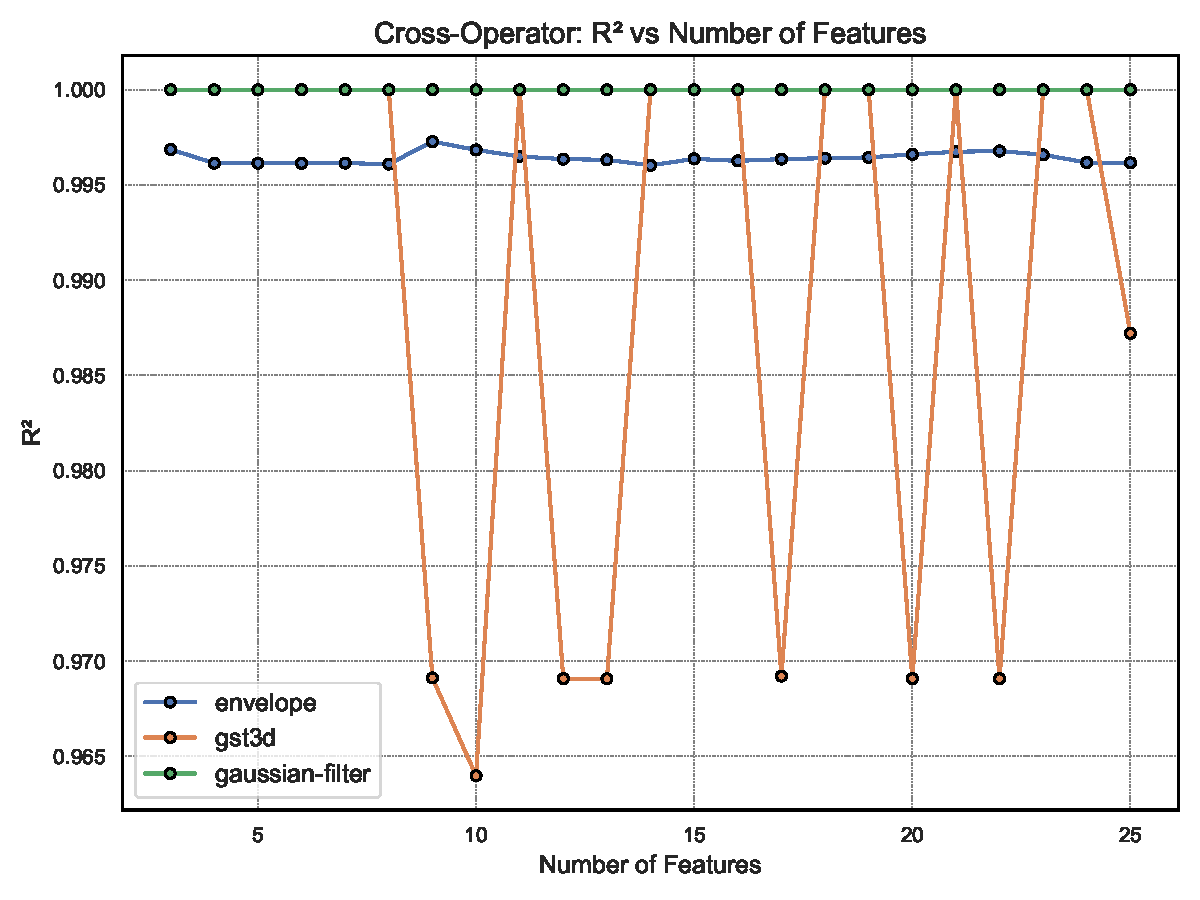
\includegraphics[width=\textwidth]{assets/images/05/cross_feature_selection_r2}
        \caption{$R^2$ changes during progressive feature removal across all operators.
        Volume stands out as indispensable.}
    \end{subfigure}
    \caption{Feature-removal impacts.
    Volume consistently emerges as the most critical input, whereas removing others typically yields negligible performance changes.}
    \label{fig:feature_selection_overview_part1}
\end{figure*}

Figure~\ref{fig:feature_selection_overview_part2} extends the analysis to residual-distribution metrics.
In particular, part~(b) shows that any small spikes in the residual curves do not substantially alter the final predictive reliability.
Hence, even simplified models (volume plus one or two shape parameters) are nearly as accurate as the full 25-feature configurations.

\begin{figure*}[htbp]
    \centering
    \begin{subfigure}[t]{0.49\textwidth}
        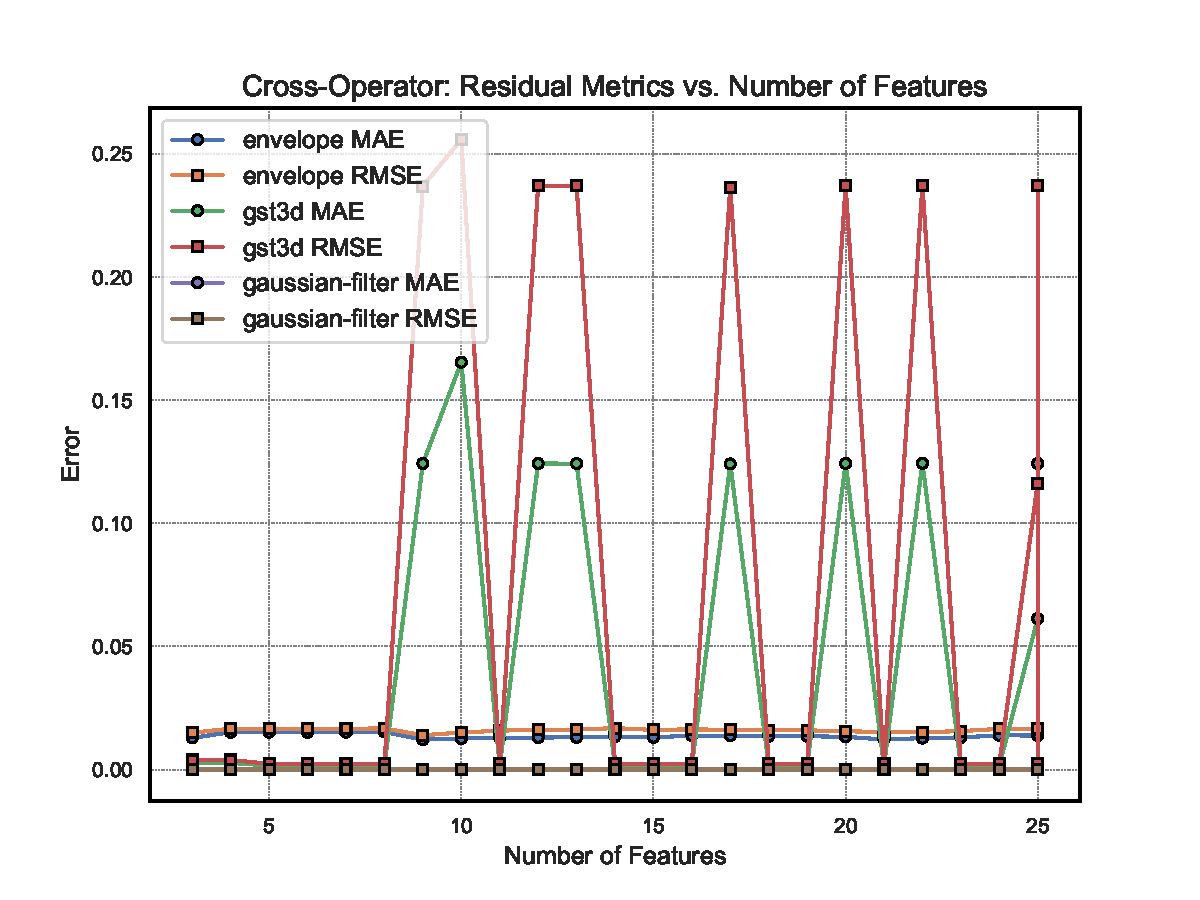
\includegraphics[width=\textwidth]{assets/images/05/residual_metrics_by_number_of_features}
        \caption{Residual-based metrics vs.\ number of features.
        Most fluctuations are minor.}
    \end{subfigure}
    \hfill
    \begin{subfigure}[t]{0.49\textwidth}
        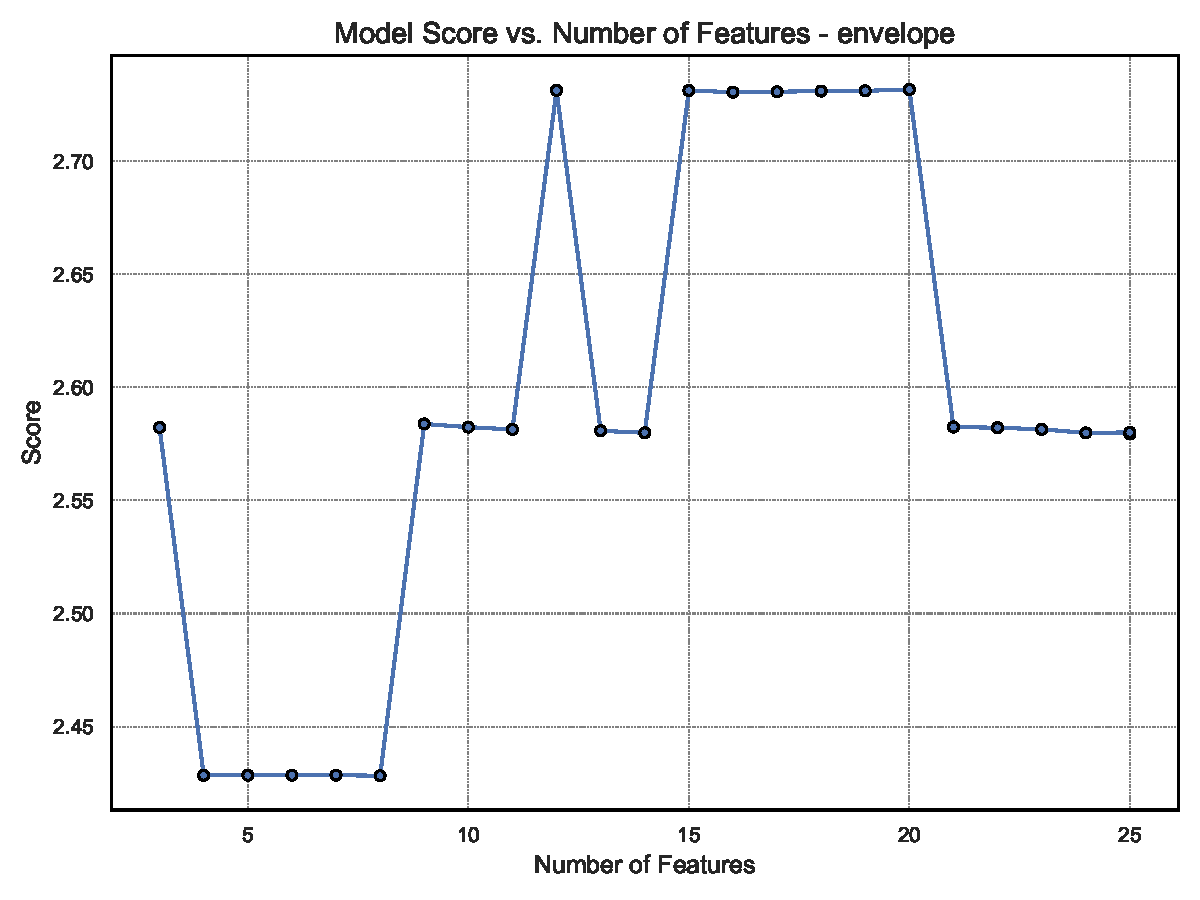
\includegraphics[width=\textwidth]{assets/images/05/score_by_number_of_features_envelope}
        \caption{Envelope example: overall “score” across successive feature removals.
        Scores remain stable or slightly improve.}
    \end{subfigure}
    \caption{Residual and score patterns under feature removal.
    Even with fewer predictors, model performance remains robust.}
    \label{fig:feature_selection_overview_part2}
\end{figure*}

\subsection{Operator-Specific Breakdown}
\label{subsec:operator-specific-breakdown}

Figures~\ref{fig:feature_impact_operator_subplots} and~\ref{fig:residual_metrics_by_number_of_features_operator_subplots} provide per-operator plots of the incremental feature-importance measurements.
The Envelope plots confirm that volume alone can achieve a \ac{RMSE} as low as 0.015.
Gaussian Filter achieves a \ac{RMSE} near \(2\times10^{-5}\) with only volume.
\ac{GST3D} benefits marginally from including another parameter (e.g., diagonal length), but dropping everything except volume still yields strong $R^2 \approx 0.9999$ in many runs.

\begin{figure*}[htbp]
    \centering
    \begin{subfigure}[t]{0.32\textwidth}
        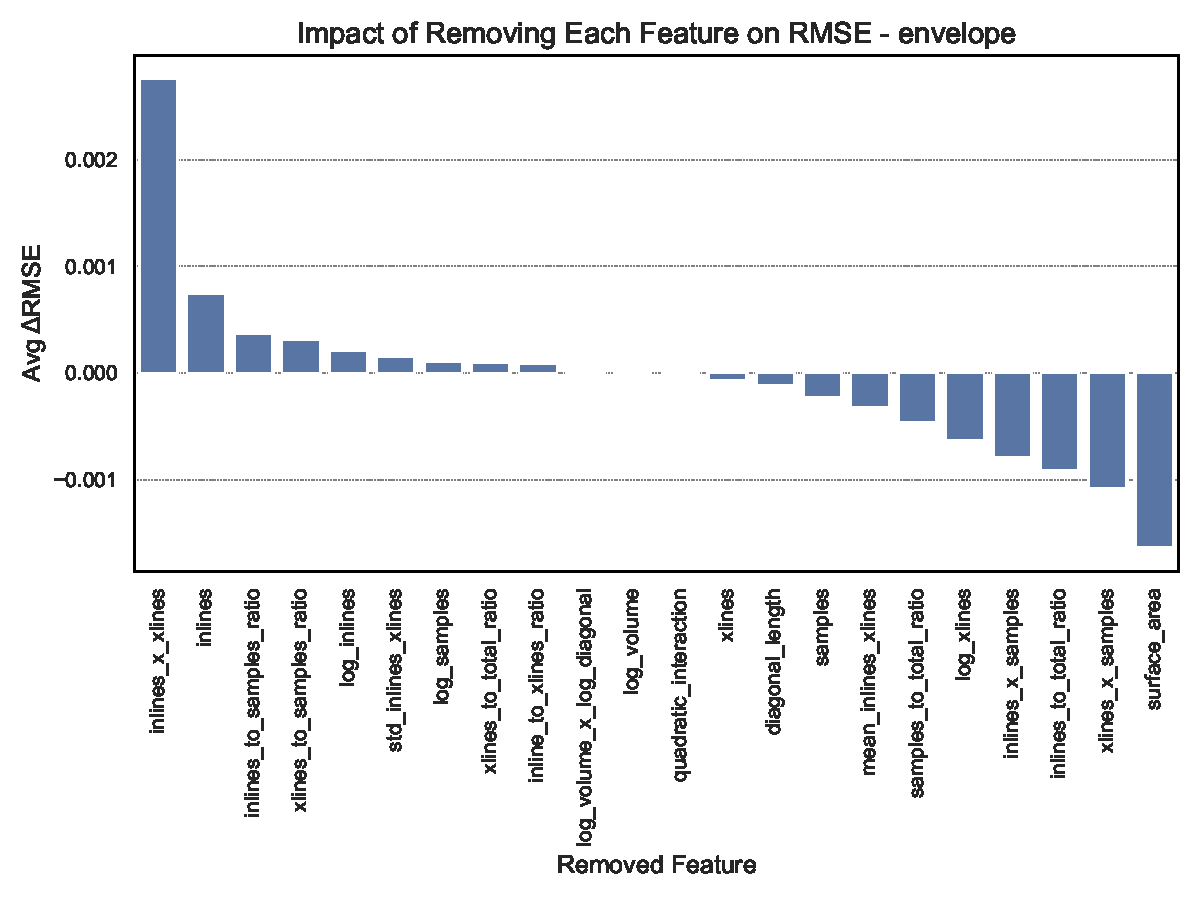
\includegraphics[width=\textwidth]{assets/images/05/feature_impact_envelope}
        \caption{Envelope}
    \end{subfigure}
    \hfill
    \begin{subfigure}[t]{0.32\textwidth}
        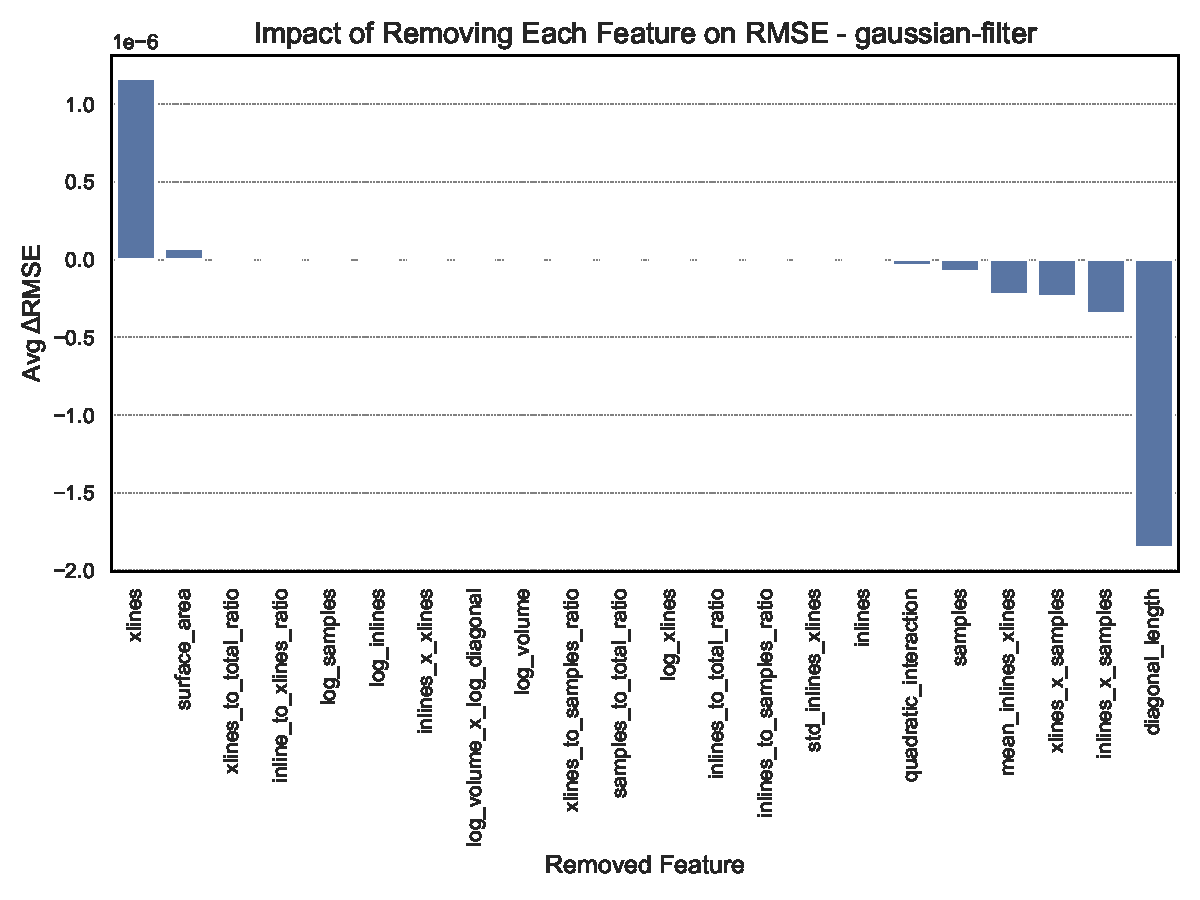
\includegraphics[width=\textwidth]{assets/images/05/feature_impact_gaussian-filter}
        \caption{Gaussian Filter}
    \end{subfigure}
    \hfill
    \begin{subfigure}[t]{0.32\textwidth}
        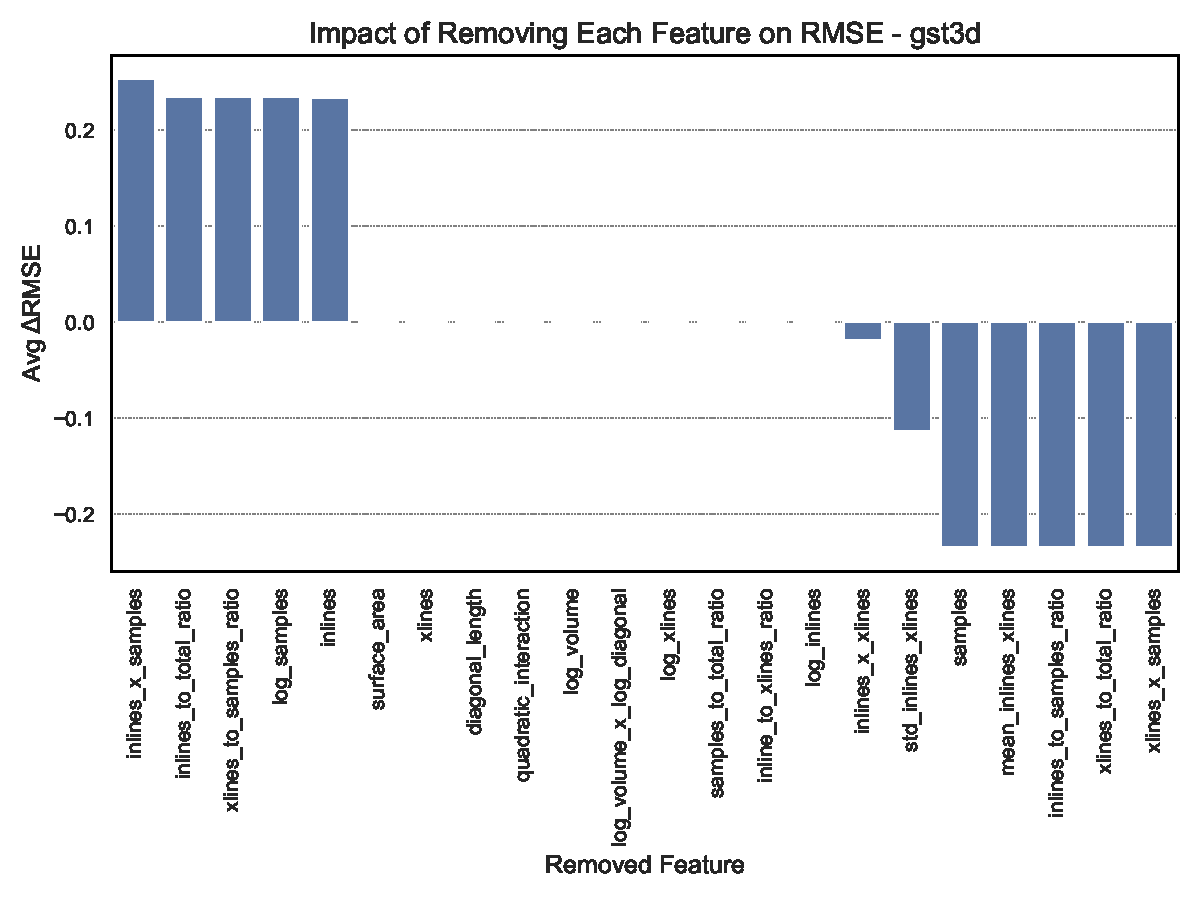
\includegraphics[width=\textwidth]{assets/images/05/feature_impact_gst3d}
        \caption{\ac{GST3D}}
    \end{subfigure}
    \caption{Feature-removal impact by operator.
    Bars represent the increase in \ac{RMSE} (or other metrics) upon discarding each feature.
    Volume is consistently the most essential.}
    \label{fig:feature_impact_operator_subplots}
\end{figure*}

\begin{figure*}[htbp]
    \centering
    \begin{subfigure}[t]{0.32\textwidth}
        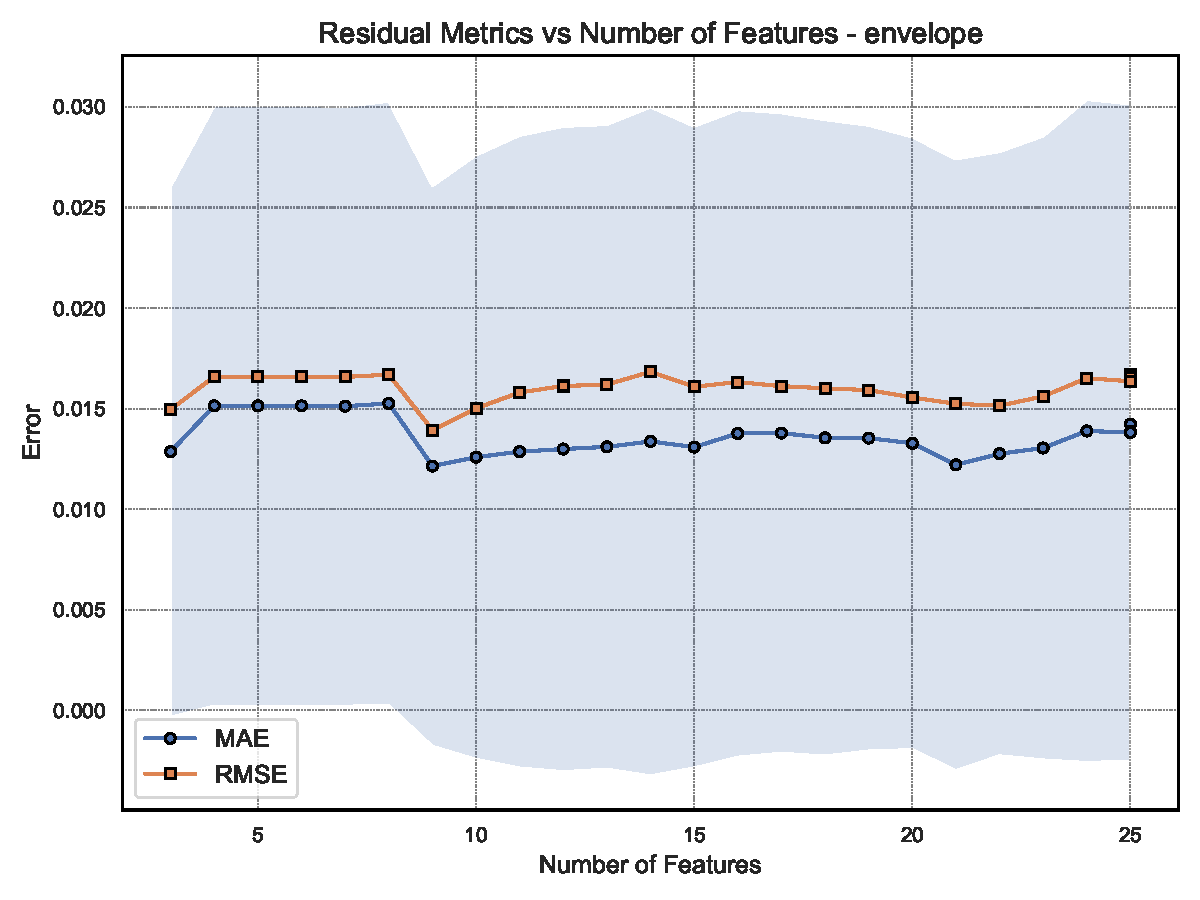
\includegraphics[width=\textwidth]{assets/images/05/residual_metrics_by_number_of_features_envelope}
        \caption{Envelope}
    \end{subfigure}
    \hfill
    \begin{subfigure}[t]{0.32\textwidth}
        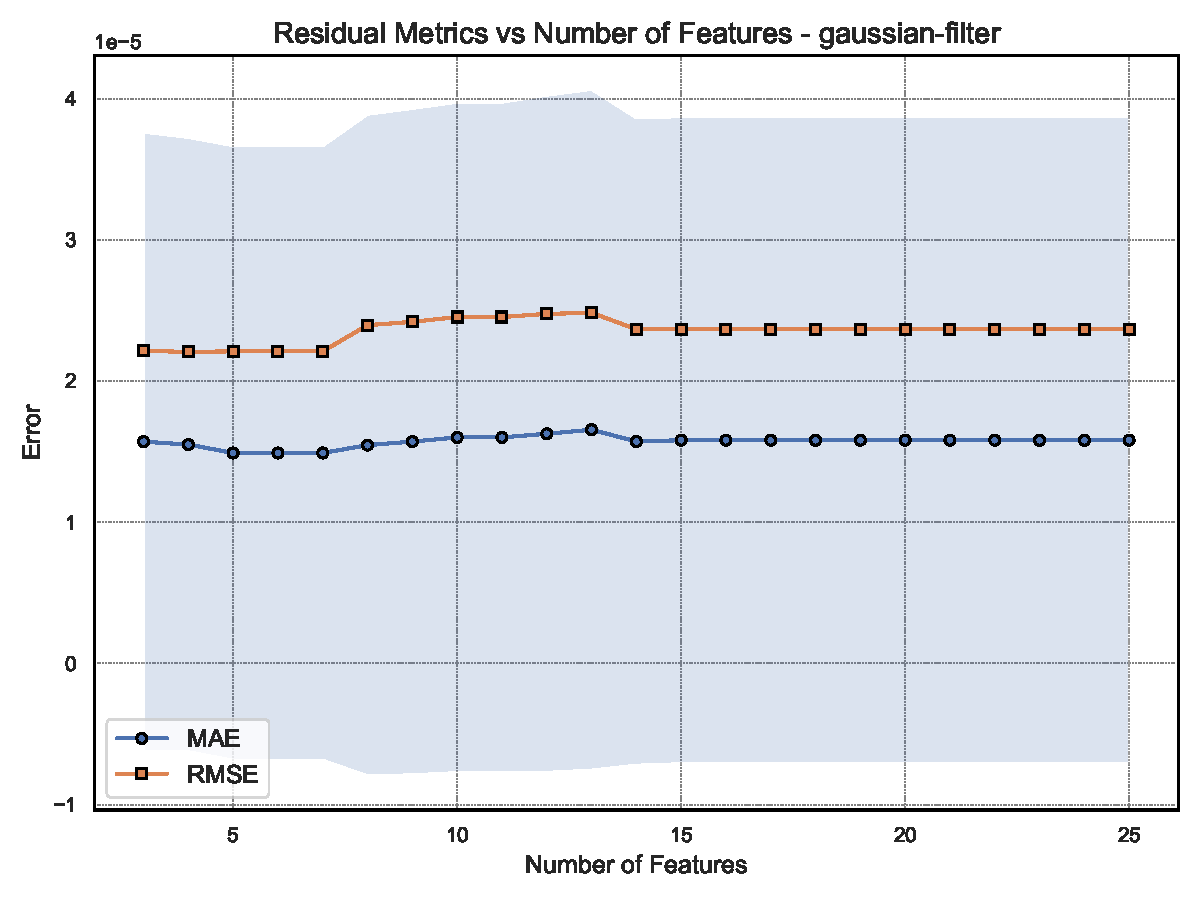
\includegraphics[width=\textwidth]{assets/images/05/residual_metrics_by_number_of_features_gaussian-filter}
        \caption{Gaussian Filter}
    \end{subfigure}
    \hfill
    \begin{subfigure}[t]{0.32\textwidth}
        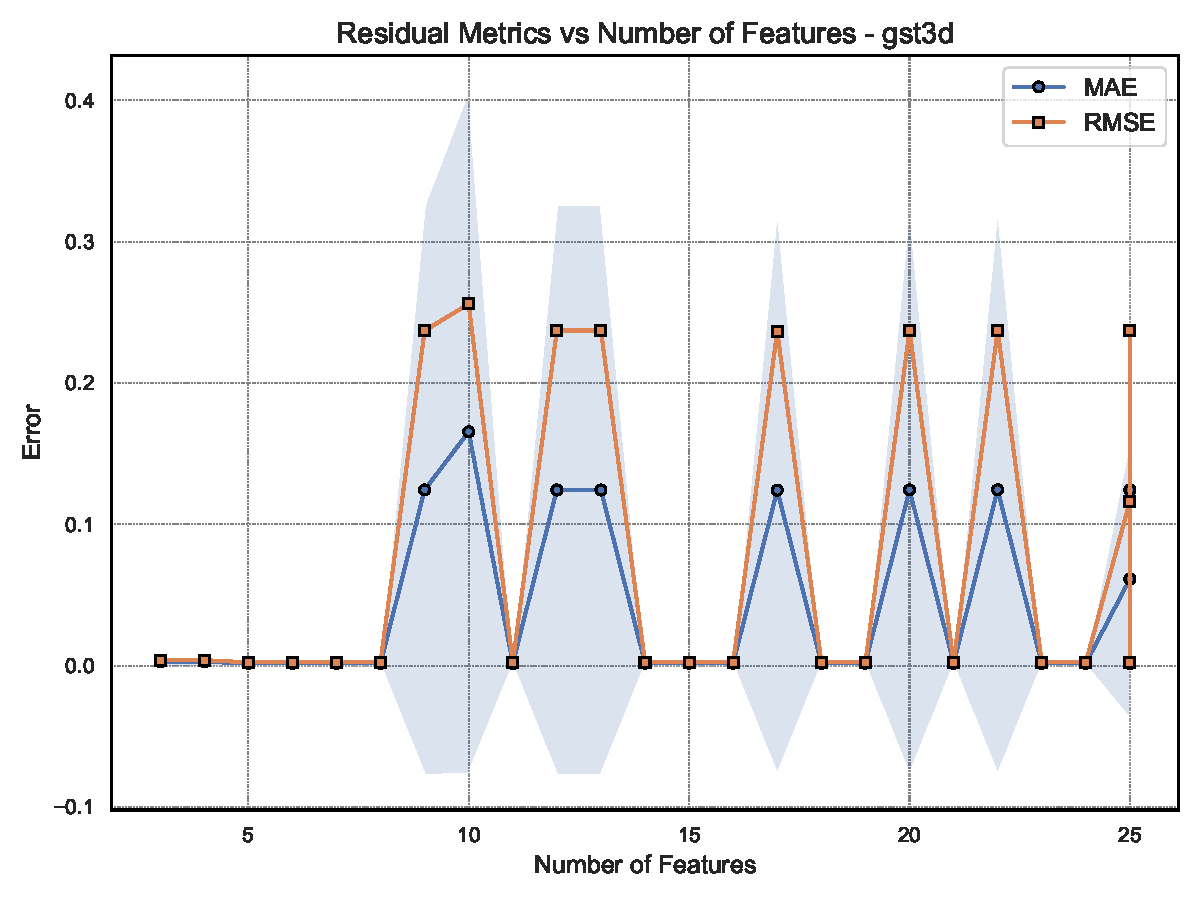
\includegraphics[width=\textwidth]{assets/images/05/residual_metrics_by_number_of_features_gst3d}
        \caption{\ac{GST3D}}
    \end{subfigure}
    \caption{Residual metrics versus number of features, split by operator.
    Envelope and Gaussian Filter are especially insensitive to feature reductions.
    \ac{GST3D} shows slightly larger performance dips when discarding non-volume inputs.}
    \label{fig:residual_metrics_by_number_of_features_operator_subplots}
\end{figure*}

\subsection{Summary of Findings}
\label{subsec:feature-selection-summary}

Collectively, these results support the conclusion that volume alone explains most memory usage variance in the tested seismic operators.
Limited improvements arise from including additional geometric attributes, yet the gain is usually minor.
Volume consistently appears in the top rank when applying \emph{SelectKBest} or other scoring schemes.
This aligns with earlier evidence of near-linear volume scaling (Section~\ref{sec:pmc-results-memory-and-execution-time-profiling}).

Practitioners seeking a lightweight memory-usage estimator can therefore rely on volume as the central input feature.
The next section investigate further data reduction (Section~\ref{sec:pmc-results-data-reduction-studies}) to refine the broader performance picture.